\documentclass[10pt]{article}
\usepackage[margin=0.7in]{geometry}\usepackage{amsmath,amssymb,tikz,hyperref}
\setlength{\parindent}{0pt}\setlength{\parskip}{5pt}
\begin{document}
\textbf{Scholten cover algebra and exceptional fibres}\hfill2026-10-31\\T-1127. Producer packet; independent source-fidelity review pending.
\section*{Checked component}
Twelve field-algebra declarations and four fixed control propositions compiled in Lean. Separate readback of all16 declarations reports only standard axioms (propositional extensionality, quotient soundness, and classical choice where used). Source/input bindings remained unchanged. No independent binary/kernel rechecker was run.

The implemented forms are $A=(1+i)t+i$, $B=(1-i)t-i$, $i^2=-1$. Checked identities include the determinant $-2i$, the quadratic leading coefficient $2i(1+x)$, conjugation exchanging $A,B$, denominator normalization, and fibre signs. In particular,
\[ A(t)^2+B(t)^2=-4t-2. \]
Thus the $x=-1$ fibre requires an infinity contribution when represented on the quintic. The checks require their stated nonzero denominators; they do not certify the Rust field implementation.
\begin{center}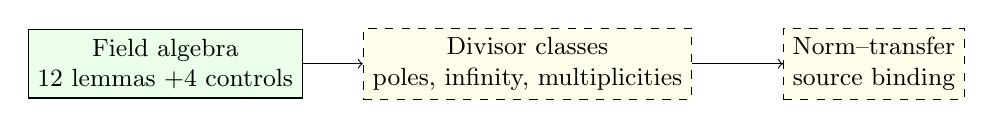
\begin{tikzpicture}[every node/.style={draw,align=center,font=\small}]
\node[fill=green!8] (a) at (0,0) {Field algebra\\12 lemmas +4 controls};
\node[dashed,fill=yellow!8] (b) at (4.6,0) {Divisor classes\\poles, infinity, multiplicities};
\node[dashed,fill=yellow!8] (c) at (9,0) {Norm--transfer\\source binding};
\draw[->] (a)--(b);\draw[->] (b)--(c);
\end{tikzpicture}\end{center}
\section*{Geometric route, conditional on class bindings}
Put $z=A/B$, $Y=y/B^3$. The two elliptic quotients are
\[f(z,Y)=(z^2,Y),\qquad g(z,Y)=(z^{-2},Y/z^3).\]
The $g$-fibre involution $(z,Y)\mapsto(-z,-Y)$ negates the $f$-image. On smooth proper models, the resulting cross push--pull maps vanish, while the diagonal degree-two compositions equal $[2]$. This gives the usual product-to-Jacobian isogeny; conjugation exchanges its factors, supplying the proposed descent from the Weil restriction.

After binding the literal divisor representatives, $f_*\tau(P)=[2]P$ implies nonzero transfer on a nonzero odd-prime-order point. A base-field isogeny then identifies the Jacobian and Weil-restriction point counts. These are written geometric deductions with explicit obligations, not conclusions certified by the twelve algebra lemmas alone.
\section*{Exceptional cases to bind}
At the quintic point at infinity, $f(\infty)=T=(-1,0)$. A degree-$d$ Mumford class pushes to $\sum f(Q_j)-dT$. The source subtracts $T$ for degree one; degree two needs no correction because $2T=O$. For $x=-1$, the finite point is $W=(-1/2,0)$ and its representative is $W-\infty$. At $B=0$, the source returns elliptic infinity. At $A=0$, ramification can give repeated roots whose multiplicities must be preserved. These source/class identifications, Cantor reduction and projective extension remain to be certified.
\section*{Evidence and sources}
The first proof attempt failed on a redundant tactic; attempt2 passed. Four controls and separate axiom readback passed, with all attempts retained. Source: \texttt{three\_leads.rs}, lines1094--1247. No scientific execution, timing, or cost ratio.

\href{https://arxiv.org/pdf/math/0312413}{Diem, genus-two covers of degree two}, Section2 and Proposition2.14, supplies classical complementary-cover context (2 invertible). \href{https://www.jmilne.org/math/CourseNotes/AV.pdf}{Milne, Abelian Varieties}, I10.20 and II1.1, supplies the characteristic-polynomial/point-count implication once an isogeny is bound. No novelty claim. Full derivation, literal obligations, hashes and statuses accompany this PDF.
\end{document}
